%%%%%%%% EACL 2027 INDUSTRY TRACK -- WORKING ANONYMOUS REVISION %%%%%%%
% Evidence-dependent items are tracked in REVISION_PLAN.md.

\documentclass[11pt]{article}

\usepackage[review]{acl}
\usepackage{times}
\usepackage{latexsym}
\usepackage[T1]{fontenc}
\usepackage[utf8]{inputenc}
\usepackage{microtype}
\usepackage{graphicx}
\usepackage{subcaption}
\usepackage{booktabs}
\usepackage{placeins}
\usepackage{amsmath}
\usepackage{amssymb}
\usepackage{mathtools}
\usepackage{amsthm}
\usepackage[capitalize,noabbrev]{cleveref}

\title{Giga-Embeddings: Mixture-of-Experts Encoders for\\High-Throughput Text Embeddings}

% Keep the review source itself anonymous.  The public preprint lists the
% authors; their names must only be restored here for the camera-ready copy.
\author{Anonymous ACL submission}

\begin{document}
\maketitle

\begin{abstract}
We introduce Giga-Embeddings, a family of text embedding models designed to combine strong retrieval quality with efficient serving.
Its largest member is a sparse 10B-parameter Mixture-of-Experts encoder that preserves substantial model capacity while activating only a fraction of it for each token.
Across English, Russian, multilingual, and code MTEB benchmarks, the MoE model achieves the strongest aggregate performance within the family on all four evaluated suites.
Under the evaluated vLLM serving configurations, its throughput is 28\%, 25\%, and 13\% higher than that of the dense 3B model at input lengths of 512, 1024, and 2048 tokens, respectively.
At 1024 tokens it reaches 114.5k tokens per second, 1.56--2.65$\times$ the throughput of the evaluated external systems.
The compact 480M model offers a Russian MTEB score comparable to FRIDA (70.96 vs.\ 70.95) with about 42\% fewer reported parameters and supports multilingual embedding tasks.
These results expose distinct quality, throughput, and storage trade-offs.
\end{abstract}

\section{Introduction}
\label{sec:introduction}

Text embeddings support semantic search, retrieval-augmented generation, clustering, classification, and semantic textual similarity.
MTEB~\citep{muennighoff2023mteb} and its multilingual expansion MMTEB~\citep{enevoldsen2025mmteb} provide broad evaluation suites for these use cases.
Recent embedding systems adapt decoder-only language models into bidirectional encoders and train them with large-scale contrastive objectives~\citep{behnamghader2024llm2vec,wang2024improving,lee2025nvembed,kolodin2025gigaembeddings}.
Although scaling the backbone generally improves representation quality, billion-parameter encoders are costly to store and serve.

Knowledge distillation offers one route to smaller encoders.
For embedding models, supervision can be transferred by matching embeddings or by matching the teacher's relative similarity scores over candidate sets~\citep{reimers2020multilingual,xu2023distillcse,zhao2026kalm}.
The latter is attractive when the teacher and student have different hidden dimensions or architectures.
It is also architecture-agnostic: a dense or sparse Mixture-of-Experts (MoE) teacher can supervise the same listwise objective through its final similarity scores.

We study a family of embedding systems that combines a high-capacity sparse encoder with smaller dense encoders, including a student trained with similarity-distribution distillation.
The 10B MoE model uses an estimated 1.63B active weights per token under the counting convention in Appendix~\ref{app:config} and exceeds the dense 3B model's measured batch-16 throughput.
The distilled 480M model targets compact deployment with Russian benchmark performance comparable to FRIDA and additional multilingual coverage.
Our contributions are:
\begin{enumerate}
  \item an openly released model family spanning dense 480M and 3B encoders and a sparse 10B encoder;
  \item a four-suite MTEB evaluation in which the 10B model has the highest reported aggregate scores within the family and the highest Russian score in our contextual external comparison;
  \item a compact encoder with a reported Russian MTEB score comparable to FRIDA (70.96 vs.\ 70.95) at about 42\% fewer parameters (480M vs.\ 823M), together with English, multilingual, and code coverage;
  \item a throughput comparison of five serving configurations in which the MoE model exceeds dense 3B throughput by 13--28\% across three input lengths. These model-level comparisons do not isolate the causal effect of sparsity.
\end{enumerate}
Direct checkpoint links are withheld during anonymous review and will be restored in the camera-ready version.

\section{Related Work}
\label{sec:related}

\paragraph{General-purpose text embeddings.}
Sentence-BERT~\citep{reimers2019sentence} and SimCSE~\citep{gao2021simcse} established bi-encoder and contrastive recipes, subsequently scaled by E5, GTE, and BGE~\citep{wang2022text,li2023towards,xiao2023cpack}.
Instruction-conditioned systems such as INSTRUCTOR, E5-Mistral, and NV-Embed~\citep{su2023instructor,wang2024improving,lee2025nvembed} adapt language models to embedding tasks.
Qwen3-Embedding~\citep{zhang2025qwen3embedding} uses the same architecture family as our dense encoders.

\paragraph{Embedding distillation.}
Classical distillation matches output distributions~\citep{hinton2015distilling}.
Representation transfer and contrastive self-distillation have been studied for sentence embeddings~\citep{reimers2020multilingual,xu2023distillcse}, while retrieval methods transfer margins or listwise similarities~\citep{hofstaetter2020improving,ren2021rocketqav2,lee2024gecko}.
KaLM-Embedding-V2 and jina-embeddings-v5-text combine contrastive supervision with distillation~\citep{zhao2026kalm,akram2026jina}.
Our recipe likewise uses an established KL objective on similarity distributions; the objective itself is not a novelty claim.

\paragraph{MoE embedding models.}
MoE models increase total capacity while activating a subset of experts per token~\citep{shazeer2017outrageously,fedus2022switch,jiang2024mixtral}.
Nomic Embed v2~\citep{nussbaum2025sparse} is a previously released general-purpose MoE text embedding model.
MoEE~\citep{li2025moee} constructs embeddings from routing weights and hidden states of existing MoE language models without additional fine-tuning.
Our study evaluates a trained bidirectional MoE encoder alongside dense models in the same released family.

\section{Model and Training Recipe}
\label{sec:method}

\begin{table}[!t]
  \caption{Core training settings; archived branch variations are detailed in Appendix~\ref{app:data}. Fine-tuning and multitask batches contain 8,192 candidate texts.}
  \label{tab:training}
  \centering
  \footnotesize
  \setlength{\tabcolsep}{1.5pt}
  \begin{tabular}{lccc}
    \toprule
    \textbf{Setting} & \textbf{Pretrain} & \textbf{Finetune} & \textbf{Multitask} \\
    \midrule
    Global batch size       & 16,384 & 1,024 & 1,024 \\
    Candidates/sample       & in-batch & 1 pos. + 7 neg. & 1 pos. + 7 neg. \\
    In-batch negatives      & yes & no & no \\
    \bottomrule
  \end{tabular}
\end{table}

\subsection{Encoder adaptation}

Following the earlier Giga-Embeddings recipe~\citep{kolodin2025gigaembeddings}, the model family adapts decoder-only language models for embedding generation.
All three encoders are initialized from proprietary GigaChat pre-training checkpoints.
The architecture-family names below describe their network designs rather than public initialization checkpoints.
The causal attention mask is replaced by a fully visible bidirectional mask, as in LLM2Vec~\citep{behnamghader2024llm2vec}, so that each token can use both left and right context.
We use mean pooling to aggregate token states into a fixed-dimensional vector and normalize the resulting vector before cosine-similarity scoring.
The instruction templates follow the earlier Giga-Embeddings recipe~\citep{kolodin2025gigaembeddings} and distinguish asymmetric retrieval inputs from symmetric semantic-similarity inputs.
The 480M, 3B, and 10B-A1.8B checkpoints and instruction set are publicly available; direct repository links are withheld during anonymous review.
The released model cards specify the MIT licence for all three checkpoints.

The 480M, 3B, and 10B-A1.8B encoders produce embeddings with dimensions 1024, 2048, and 1536, respectively.
The 480M and 3B models use dense bidirectional encoders in the Qwen3 architecture family~\citep{zhang2025qwen3embedding}, while the largest model is a bidirectional DeepSeekMoE-style encoder~\citep{dai2024deepseekmoe} with 10B total parameters, 64 routed experts, one shared expert, and top-4 routing.
The dense encoders have 28 and 36 layers with hidden sizes 1024 and 2048; the MoE encoder has 26 layers with hidden size 1536, sigmoid router scores, and 1280-dimensional expert feed-forward layers.
We retain the released model identifier ``10B-A1.8B''; our explicit active-weight estimate is approximately 1.63B, as detailed with the checkpoint configurations in Appendix~\ref{app:config}.
% Pending author confirmation: exact initialization checkpoint revisions,
% training-time balancing objective, token-dropping policy, and merging.
We use ``480M'', ``3B'', and ``10B-A1.8B'' as short model-family names.

\subsection{Three-stage contrastive training}

As in the first Giga-Embeddings release~\citep{kolodin2025gigaembeddings}, training has three stages: broad contrastive pre-training, retrieval fine-tuning with hard negatives, and multitask fine-tuning for retrieval, classification, clustering, and semantic similarity.
Embedding training uses open-source data from the Nemotron~\citep{babakhin2025nemotron} and KaLM~\citep{zhao2026kalm} recipes.
Appendix~\ref{app:data} identifies the corresponding public source collections and their published roles.
The proprietary component is the GigaChat backbone pre-training, whereas the embedding-stage data are open-source.
% Exact consumed dataset revisions and final-release merge lineage remain
% incomplete; recovered compact-run counts are reported in the appendix.
Across all stages, the learning rate starts at $3\times10^{-5}$ and follows a cosine decay schedule with a 1\% warmup fraction and a minimum learning rate of $10^{-7}$.
We use weight decay of 0.01, Adam coefficients $\beta_1=0.9$ and $\beta_2=0.999$, and an InfoNCE temperature of 0.02.
Fine-tuning runs for one epoch and multitask training for three epochs.
The stage-specific settings are summarized in \Cref{tab:training}.
The recovered compact F2LLM pre-training branch uses global batch 1024 rather than the core pre-training value 16,384; its membership in the final merge is not established.

Our contrastive-loss formulation follows Qwen3-Embedding~\citep{zhang2025qwen3embedding}.
Pre-training uses in-batch InfoNCE, includes query--query and document--document contrastive terms, and masks detected false negatives.
Fine-tuning and multitask training disable in-batch negatives and use the explicit eight-candidate groups described in \Cref{tab:training}.
For a batch of $B$ queries, let $\mathcal{C}_i$ be the fixed candidate set for query $q_i$, let $p(i)$ index its positive candidate, and let $s_{ij}$ be the student cosine similarity.

\begin{figure*}[!t]
  \centering
  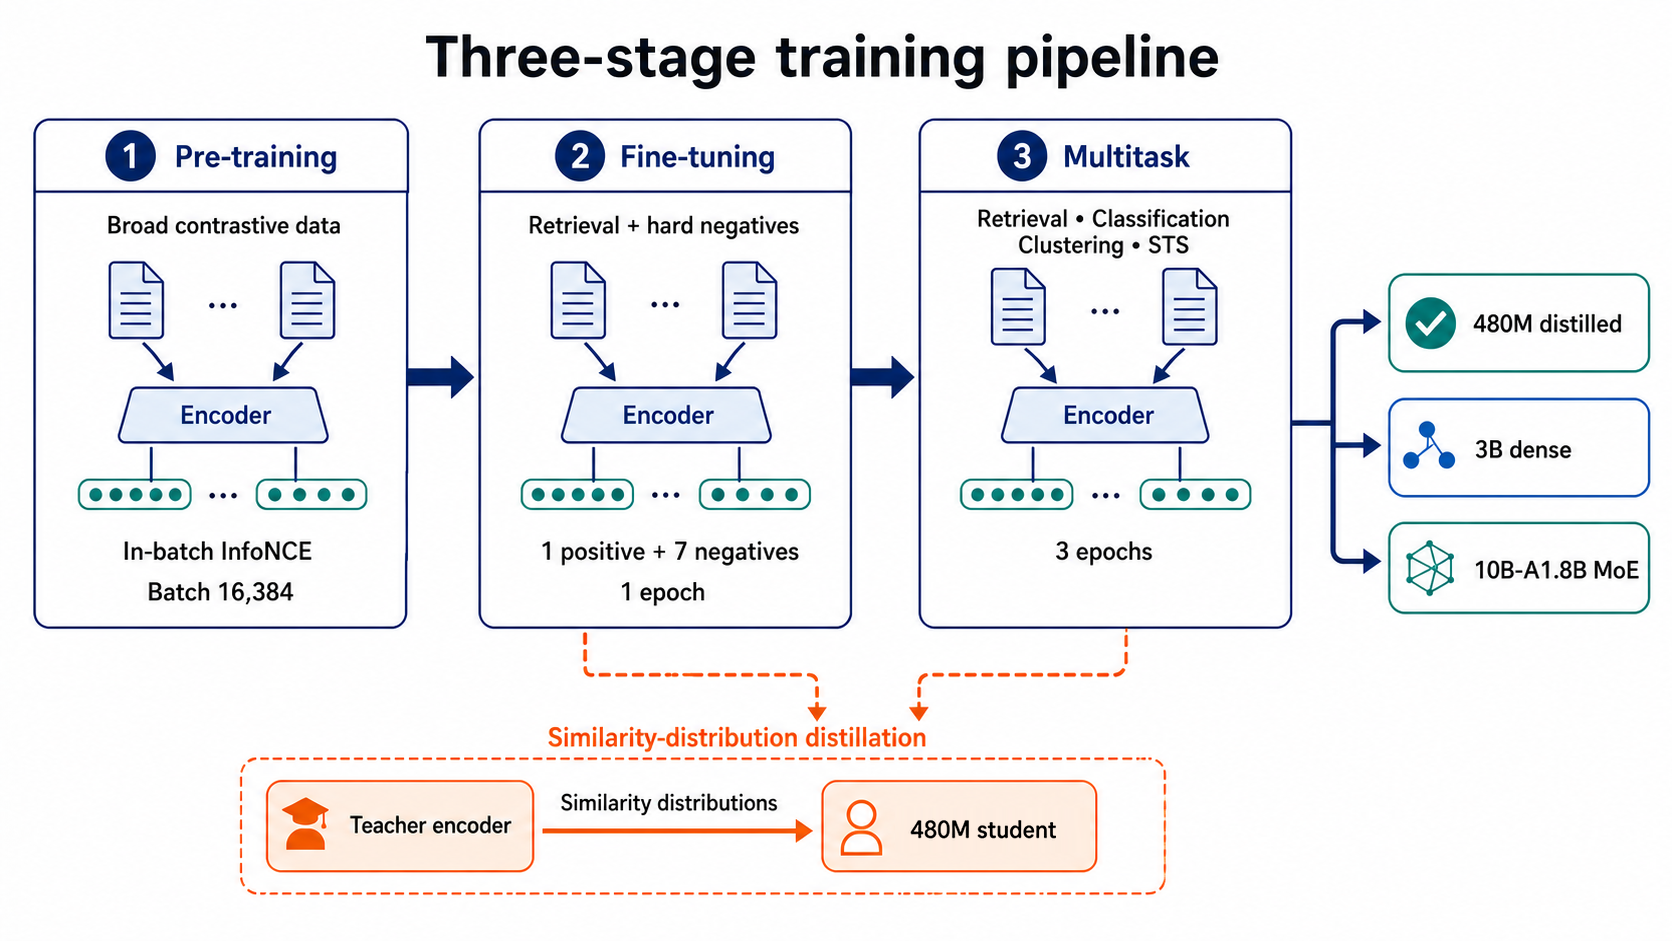
\includegraphics[width=0.90\textwidth]{figures/training_pipeline_gpt_image_2.png}
  \caption{Core three-stage embedding training pipeline. All models undergo contrastive pre-training, retrieval fine-tuning, and multitask fine-tuning. During the latter two stages, only the 480M student additionally matches similarity distributions from a 10B MoE teacher.}
  \label{fig:training-pipeline}
\end{figure*}

\begin{samepage}
We use batch-mean InfoNCE~\citep{oord2018representation}:
\begin{equation}
  \mathcal{L}_{\mathrm{NCE}} = -\frac{1}{B}\sum_{i=1}^{B}
  \log \frac{\exp(s_{i,p(i)}/\tau)}
  {\sum_{j \in \mathcal{C}_i}\exp(s_{ij}/\tau)}.
  \label{eq:nce}
\end{equation}
\end{samepage}
Hard negatives for retrieval fine-tuning are mined from a predefined retrieval-rank range.

\subsection{Similarity-distribution distillation}
\label{sec:distill}

We apply similarity-distribution distillation exclusively to the 480M model during retrieval fine-tuning and multitask fine-tuning.
The teacher is a 10B MoE encoder initialized from a proprietary GigaChat pre-training checkpoint.
Teacher query and candidate vectors are precomputed and cached; training forms similarity targets from these vectors rather than executing the teacher online.
% Teacher architecture confirmed by the authors; exact checkpoint revision
% and its identity relative to the evaluated 10B release remain to be pinned.
Its pre-training stage uses only the contrastive objective, and the 3B and 10B-A1.8B models are trained without distillation.
For both distilled stages, $\lambda=0.3$, $\tau_{\mathrm{KD}}=0.05$, and the contrastive temperature is 0.02.
Because the objective aligns distributions over query--candidate similarity scores rather than embedding coordinates, the teacher and student may use different embedding dimensions.
By contrast, direct MSE or cosine-similarity alignment between teacher and student embedding vectors requires equal dimensions or an additional learned projection.
Let $t_{ij}$ be the teacher cosine similarity for the same support $\mathcal{C}_i$.
Teacher and student distributions are
\begin{align}
P_T(j\mid q_i) &= \frac{\exp(t_{ij}/\tau_{\mathrm{KD}})}
 {\sum_{k\in\mathcal{C}_i}\exp(t_{ik}/\tau_{\mathrm{KD}})}, \\
P_S(j\mid q_i) &= \frac{\exp(s_{ij}/\tau_{\mathrm{KD}})}
 {\sum_{k\in\mathcal{C}_i}\exp(s_{ik}/\tau_{\mathrm{KD}})}.
\end{align}
The distillation term is a batch mean over identical supports:
\begin{equation}
  \mathcal{L}_{\mathrm{KD}} = \frac{1}{B}\sum_{i=1}^{B}
  D_{\mathrm{KL}}\!\left(P_T(\cdot\mid q_i)\,\|\,P_S(\cdot\mid q_i)\right).
  \label{eq:kd}
\end{equation}
The combined objective is
\begin{equation}
  \mathcal{L}=\lambda\mathcal{L}_{\mathrm{KD}}
  +(1-\lambda)\mathcal{L}_{\mathrm{NCE}}.
  \label{eq:combined}
\end{equation}
The KL term transfers the teacher's relative similarity structure over each candidate set, while InfoNCE preserves direct contrastive supervision.
Because the loss depends only on final similarity scores, it does not require access to the teacher's internal architecture or routing decisions.

% Evaluation tables are declared here so they appear near the section without
% interrupting the text flow below the single-column training table.
\begin{table*}[!t]
  \centering
  \begin{minipage}[t]{0.35\textwidth}
    \vspace{0pt}
    \captionof{table}{Model architectures; active counts follow Appendix~\ref{app:config}.}
    \label{tab:architecture}
    \centering
    \small
    \setlength{\tabcolsep}{3.2pt}
    \begin{tabular}{lrrr}
      \toprule
      \textbf{Type} & \textbf{Total} & \textbf{Active} & \textbf{Dim.} \\
      \midrule
      Dense      & 480M & 480M & 1024 \\
      Dense      & 3B & 3B & 2048 \\
      MoE        & 10B & $\sim$1.63B & 1536 \\
      \bottomrule
    \end{tabular}
  \end{minipage}
  \hfill
  \begin{minipage}[t]{0.62\textwidth}
    \vspace{0pt}
    \captionof{table}{MTEB scores (\%). Leaderboard \texttt{meanTask}, 2026-10-29. $\dagger$: reaggregated archive (Appendix~\ref{app:multilingual}). Bold: family maximum.}
    \label{tab:main}
    \centering
    \small
    \setlength{\tabcolsep}{3.5pt}
    \begin{tabular}{rrrrrr}
      \toprule
      \textbf{Scale} & \textbf{Dim.} & \textbf{English} & \textbf{Russian} & \textbf{Multilingual} & \textbf{Code} \\
      \midrule
      480M       & 1024 & 69.52 & 70.96 & 56.80$^{\dagger}$ & 72.87 \\
      3B         & 2048 & 71.90 & 74.55 & 63.89 & 76.94 \\
      10B-A1.8B  & 1536 & \textbf{72.23} & \textbf{74.99} & \textbf{65.64} & \textbf{78.43} \\
      \bottomrule
    \end{tabular}
  \end{minipage}
\end{table*}

\begin{table*}[!t]
  \caption{Offline token-ID throughput (tokens/s): one H100 80~GB per run, vLLM 0.24.0, BF16, batch 16. Seven timed repeats after three warm-ups; relative: MoE $=1$ at 1024 tokens.}
  \label{tab:throughput}
  \centering
  \small
  \setlength{\tabcolsep}{5pt}
  \begin{tabular}{p{8.0cm}rrrr}
    \toprule
    \textbf{Model (vLLM)} & \textbf{512 tokens} & \textbf{1024 tokens} & \textbf{2048 tokens} & \textbf{Relative} \\
    \midrule
    Qwen3-Embedding-4B
      & 70.1k & 73.2k & 71.2k & 0.64$\times$ \\
    F2LLM-v2-8B
      & 43.2k & 43.4k & 42.6k & 0.38$\times$ \\
    nvidia/llama-embed-nemotron-8b
      & 42.6k & 43.2k & 41.7k & 0.38$\times$ \\
    \midrule
    \textbf{Ours: 3B}
      & 87.9k & 91.5k & 90.4k & 0.80$\times$ \\
    \textbf{Ours: 10B-A1.8B}
      & \textbf{112.6k} & \textbf{114.5k} & \textbf{102.3k} & \textbf{1.00$\times$} \\
    \bottomrule
  \end{tabular}
\end{table*}

% Queue the two wide external-comparison tables early enough to place them at
% the top of the final main-text page instead of leaving a sparse preceding page.
\begin{table*}[!t]
  \caption{Contextual comparison with compact models on MTEB benchmark suites (\%). Public baselines use official MTEB Leaderboard \texttt{meanTask} values retrieved on 2026-08-08; our result is from \Cref{tab:main}. Scores use different evaluation settings; a dash denotes an unavailable score.}
  \label{tab:baselines}
  \centering
  \small
  \setlength{\tabcolsep}{5pt}
  \begin{tabular}{lrrcccc}
    \toprule
    \textbf{Model} & \textbf{Params} & \textbf{Dim.} & \textbf{Russian} & \textbf{English} & \textbf{Multilingual} & \textbf{Code} \\
    \midrule
    sergeyzh/BERTA                              & 128M & 768  & 69.39 & --- & --- & --- \\
    google/embeddinggemma-300m                  & 308M & 768  & 65.19 & 69.67 & 61.15 & 68.76 \\
    codefuse-ai/F2LLM-v2-0.6B                   & 596M & 1024 & 65.97 & 69.97 & 62.74 & 77.41 \\
    Qwen/Qwen3-Embedding-0.6B                   & 596M & 1024 & 64.29 & 70.47 & 64.34 & 75.42 \\
    ai-forever/FRIDA                            & 823M & 1536 & 70.95 & --- & --- & --- \\
    \midrule
    \textbf{Ours: 480M}                         & 480M & 1024 & 70.96 & 69.52 & 56.80$^{\dagger}$ & 72.87 \\
    \bottomrule
  \end{tabular}
\end{table*}

\begin{table*}[!t]
  \caption{Contextual comparison with larger models on MTEB benchmark suites (\%). Public baselines use official MTEB Leaderboard \texttt{meanTask} values retrieved on 2026-08-08; our results are from \Cref{tab:main}. Scores use different evaluation settings.}
  \label{tab:large-baselines}
  \centering
  \small
  \setlength{\tabcolsep}{4.5pt}
  \begin{tabular}{lrrcccc}
    \toprule
    \textbf{Model} & \textbf{Params} & \textbf{Dim.} & \textbf{Russian} & \textbf{English} & \textbf{Multilingual} & \textbf{Code} \\
    \midrule
    codefuse-ai/F2LLM-v2-1.7B                              & 1.72B  & 2048 & 68.52 & 71.63 & 65.21 & 78.76 \\
    codefuse-ai/F2LLM-v2-4B                                & 4.02B  & 2560 & 69.46 & 72.41 & 67.06 & 80.15 \\
    Qwen/Qwen3-Embedding-4B                                & 4.02B  & 2560 & 70.13 & 74.61 & 69.45 & 80.07 \\
    Qwen/Qwen3-Embedding-8B                                & 7.57B  & 4096 & 71.42 & 75.23 & 70.58 & 80.69 \\
    codefuse-ai/F2LLM-v2-8B                                & 7.57B  & 4096 & 70.57 & 72.86 & 68.09 & 80.16 \\
    codefuse-ai/F2LLM-v2-14B                               & 13.99B & 5120 & 70.90 & 73.08 & 68.74 & 80.75 \\
    \midrule
    \textbf{Ours: 3B}                                      & 3B     & 2048 & 74.55 & 71.90 & 63.89 & 76.94 \\
    \textbf{Ours: 10B-A1.8B}                               & 10B    & 1536 & 74.99 & 72.23 & 65.64 & 78.43 \\
    \bottomrule
  \end{tabular}
\end{table*}

\section{Evaluation}
\label{sec:evaluation}

\subsection{Evaluation protocol}

For the released checkpoints, we report the official MTEB Leaderboard's benchmark-level \texttt{meanTask} aggregates retrieved on 2026-10-29.
The four suites contain 41 English, 23 Russian, 131 multilingual, and 12 code tasks; each task receives equal weight in the suite-level mean.
The Russian suite follows ruMTEB~\citep{snegirev2025rumteb}, while the multilingual suite follows MMTEB~\citep{enevoldsen2025mmteb}.
The public snapshot has no complete multilingual aggregate for 480M.
Its $\dagger$ value is a CPU reaggregation of an archived, mixed-version score cache attributed to that model, not a new inference run or an independently checkpoint-linked public score.
This gives 56.80; the earlier 56.97 is withdrawn because the recovered notebook has a stale-score aggregation defect (Appendix~\ref{app:multilingual}).
The distillation comparison retains the original run-level ablation scores and is reported separately from these public-release aggregates.
For 480M Russian, the original 70.98 and public 70.96 are reproducible from identical task results: test-preferred averaging gives 70.978526, whereas including validation and test for the two MASSIVE tasks gives 70.959130 (Appendix~\ref{app:aggregation}).

At two bytes per weight (BF16 or FP16), the 480M, 3B, and 10B-A1.8B models require approximately 0.97, 6.30, and 20.95~GB of weight storage, respectively (decimal GB).
The distilled model therefore uses about 4.6\% as much weight storage as the MoE model.
These theoretical estimates exclude activations and other runtime state.

\subsection{Aggregate results}

\Cref{tab:main} presents task-macro scores for all three models.
The 480M distilled model reaches 69.52 on English, 70.96 on Russian, and 72.87 on Code in the public snapshot; its reaggregated archived Multilingual value is 56.80.
Using the underlying, unrounded public aggregates, its English, Russian, and Code gaps to 3B are 2.39, 3.59, and 4.07 points.
The Multilingual gap is approximately 7.09 points using the archived value, subject to the checkpoint-linkage limitation above.

The 10B-A1.8B model achieves the highest score within the family on every benchmark.
Using unrounded public aggregates, the differences from 3B are +0.33 on English, +0.43 on Russian, +1.75 on Multilingual, and +1.49 on Code.
Because each model is evaluated once, the sub-one-point differences on English and Russian should be interpreted cautiously.

\subsection{Descriptive distillation comparison}

\begin{table}[!t]
  \caption{Original single-run training variants (\%). Differences in initialization and microbatch size prevent interpreting this as a matched KD-only control.}
  \label{tab:distillation-ablation}
  \centering
  \small
  \setlength{\tabcolsep}{3.5pt}
  \begin{tabular}{lrrr}
    \toprule
    \textbf{Model} & \textbf{English} & \textbf{Russian} & \textbf{Code} \\
    \midrule
    480M, no distillation & 69.43 & 70.86 & 72.65 \\
    480M, distilled       & 69.52 & 70.98 & 72.87 \\
    \bottomrule
  \end{tabular}
\end{table}

\Cref{tab:distillation-ablation} reports two single-run 480M training variants, using the original test-preferred Russian aggregation.
The observed English, Russian, and Code differences are +0.09, +0.12, and +0.22 points, respectively.
Recovered records name different merged starting checkpoints and microbatch sizes (128 with KD, 64 without), although both use global batch 1024.
The current initialization files differ in 308 of 310 tensors; their historical training-time hashes were not retained.
Training-row identity, historical inference settings, and merge equivalence are not established, so these differences do not isolate a causal KD effect.
No multilingual no-KD result or repeated-seed series was recovered.

\subsection{Inference throughput}

Recovered timings use one H100 80~GB HBM3 per run, BF16, and vLLM 0.24.0.
Inputs are synthetic random token IDs of exact length, without padding; each cell has three warm-ups and seven synchronous timed repeats.
Throughput is $BL$ divided by median encode-call wall time, excluding model loading, tokenization, and input generation.
The script, software versions, configuration differences, and checkpoint-linkage scope are detailed in Appendix~\ref{app:serving}.

The MoE configuration has the highest throughput among the five configurations in \Cref{tab:throughput} at each evaluated length.
Relative to dense 3B, its throughput is 1.28$\times$, 1.25$\times$, and 1.13$\times$ as high at 512, 1024, and 2048 tokens, respectively.
All five configurations use vLLM; their architecture and engine-profile differences prevent isolating the contribution of sparse activation or establishing an equal-quality advantage.
The 480M model is outside this throughput comparison; its estimated 16-bit weight storage is 0.97~GB, which describes model size rather than runtime efficiency.
Latency and peak GPU memory are not reported in this comparison.

\subsection{External baseline comparison}

\Cref{tab:baselines,tab:large-baselines} compare Giga-Embeddings with public results from the \href{https://huggingface.co/spaces/mteb/leaderboard}{MTEB Leaderboard}.
Differences in prompts and evaluation settings make these contextual rather than controlled same-run comparisons.
Our 10B-A1.8B model has the highest reported Russian score in this comparison, while Qwen3-Embedding-8B has the highest English and Multilingual scores and F2LLM-v2-14B the highest Code score.
Qwen3-Embedding-4B also scores higher than our MoE model on English, Multilingual, and Code; the throughput comparison therefore does not establish an advantage at equal embedding quality.
The compact model illustrates parameter efficiency at comparable reported Russian quality: it scores 70.96 against FRIDA's 70.95 with about 42\% fewer parameters, using the reported model sizes of 480M and 823M.
The same checkpoint also supports English, multilingual, and code embedding tasks.

\section{Conclusion}

We present Giga-Embeddings, a family of dense and sparse bidirectional text encoders.
The 10B-A1.8B model has the highest reported aggregate scores within the family on four MTEB suites and 13--28\% higher measured batch-16 throughput than the dense 3B model.
The MoE configuration is fastest among the five configurations in the throughput table, while its larger full checkpoint requires more weight storage than dense 3B.
The external comparisons show a quality trade-off: the MoE model has a higher reported Russian score, whereas Qwen3-Embedding-4B has higher English, Multilingual, and Code scores.
The 480M model combines a reported Russian MTEB score comparable to FRIDA with about 42\% fewer parameters and additional multilingual coverage.
Together, the checkpoints illustrate distinct trade-offs between benchmark performance, measured token throughput, and model storage for embedding workloads.

\section{Limitations}

Our benchmark results report a single run per model, so small score differences do not have uncertainty estimates.
Throughput results use synthetic token IDs on one GPU SKU across separate sessions, with seven timed repeats per setting.
The comparison omits the 480M model and does not report latency or peak GPU memory; theoretical weight storage is a separate model-size estimate.
Engine profiles differ, so the throughput advantage cannot be attributed solely to sparsity.
The backbone pre-training checkpoints are proprietary, which limits reproduction from raw data.
Preserved records do not establish complete initialization, teacher-cache, and merge lineage, or the historical MoE balancing objective.
We report no overlap between embedding-training and evaluation examples; a detailed record of the checking procedure was not located in the inspected artifacts.
The KD comparison has training and packaging confounds and does not establish a causal distillation gain.
The 480M Multilingual value is reaggregated from an archived mixed-version cache without an immutable checkpoint binding.
Finally, aggregate MTEB scores can hide variation across individual tasks and languages.
Future evaluations should include matched controls, frozen evaluation provenance, and natural-text workloads across serving configurations.

\FloatBarrier
\bibliography{references_revised}

\appendix
\section{Released Checkpoint Configurations}
\label{app:config}

The public release configurations specify 28 layers, hidden size 1024, feed-forward size 3072, 16 attention heads, 8 key/value heads, and head dimension 64 for the 480M encoder.
The 3B encoder has 36 layers, hidden size 2048, feed-forward size 11008, 16 attention heads, 8 key/value heads, and head dimension 128.
Both use the Qwen3 bidirectional architecture family and a vocabulary of 128,256 tokens.

The MoE encoder uses the DeepSeek-V3 bidirectional architecture family with 26 layers, hidden size 1536, 32 attention heads, and the same vocabulary size.
Its first layer has a dense feed-forward block of intermediate size 8960; the remaining 25 layers use 64 routed experts with intermediate size 1280, top-4 selection, and one shared expert.
The released router configuration specifies sigmoid scores, \texttt{noaux\_tc} selection, one expert group, normalization of selected routing weights, and a routing scale of 1.0.
Multi-head latent attention uses a key/value low-rank dimension of 512, non-rotary and rotary query/key head dimensions of 128 and 64, and a value-head dimension of 192.
These are release-configuration settings; the router implementation name alone does not establish the training-time balancing objective.

The released safetensors metadata give total parameter counts of 483,717,632, 3,150,605,312, and 10,475,534,400 for the 480M, 3B, and MoE models, respectively.
The MoE routed expert matrices contain
\begin{align}
N_{\mathrm{routed}} &= 25\cdot64\cdot3\cdot1536\cdot1280 \notag\\
&= 9{,}437{,}184{,}000.
\end{align}
weights, accounting for the gate, up, and down projections of each expert.
Our active-weight estimate counts all non-routed weights, including shared experts and the embedding table, plus four of the 64 routed experts per token:
\begin{align}
N_{\mathrm{active}} &= N_{\mathrm{total}}-N_{\mathrm{routed}}
 +\frac{4}{64}N_{\mathrm{routed}} \\
&=1{,}628{,}174{,}400.
\end{align}
This convention estimates active weights rather than FLOPs, GPU residency, or peak memory.

\section{Public Training Data Sources}
\label{app:data}

The source recipes are Nemotron~\citep{babakhin2025nemotron} and KaLM~\citep{zhao2026kalm}.
KaLM publishes a \href{https://huggingface.co/datasets/HIT-TMG/KaLM-embedding-pretrain-data}{pre-training collection (HIT-TMG)} and a \href{https://huggingface.co/datasets/KaLM-Embedding/KaLM-embedding-finetuning-data}{fine-tuning collection (KaLM-Embedding)}.
The Nemotron report describes a retrieval-pretraining mixture derived from Nemotron-CC-v2 and a separate fine-tuning mixture; its public fine-tuning release is \href{https://huggingface.co/datasets/nvidia/embed-nemotron-dataset-v1}{Embed Nemotron Dataset V1}.
These references identify the public source collections and distinguish their published roles; their published sizes are not estimates of our post-filtering stage-specific sample counts.

Recovered experiment manifests list 25 KaLM pre-training files, 62 KaLM fine-tuning files, 14 Nemotron fine-tuning files, and 123 inputs in one multitask manifest.
The 14 Nemotron entries are EmotionClassification, FEVER, GooAQ, HotpotQA, MAmmoTH2, MIRACL, MSMARCO, NaturalQuestions, NFCorpus, PAQ, SciFact, SQuAD, SyntheticClassificationData, and TriviaQA.
Additional manifests describe earlier-recipe and F2LLM branches, but the full merge lineage establishing which branches enter each final release was not recovered.
These counts describe file inventories, not example counts or independently verified release mixtures.
\Cref{tab:prepared-counts} adds prepared-dataset sizes reported in preserved compact-model logs and consumed-sample counters recovered from their checkpoints.
Prepared rows are the logged dataset size after preparation; consumed samples include repeated epochs and are not unique-example counts.
These measurements describe particular development branches rather than a reconstructed final-release mixture.
The multitask row belongs to a completed August~3 run, not the missing August~4 KD or August~7 no-KD checkpoints.
KaLM fine-tuning counts are confirmed for no-KD and a separate KaLM-12B-teacher run, not the missing 10B-teacher log.
Giga and F2LLM have completed compact training branches, but executed merges linking all branch outputs to each release remain unverified.

\begin{table}[t]
  \caption{Archived compact-model training counts. Prepared rows and consumed samples have different meanings; rows must not be summed as a unique final training mixture.}
  \label{tab:prepared-counts}
  \centering
  \footnotesize
  \setlength{\tabcolsep}{3pt}
  \begin{tabular}{lrr}
    \toprule
    \textbf{Branch/stage} & \textbf{Prepared rows} & \textbf{Consumed} \\
    \midrule
    Giga pretrain     & 91,030,382 & 91,029,504 \\
    KaLM pretrain     & 299,034,744 & 299,024,384 \\
    F2LLM pretrain    & 10,597,526 & 10,597,376 \\
    Giga finetune     & 1,131,959 & 1,131,520 \\
    Nemotron finetune & 3,355,596 & 3,354,624 \\
    KaLM finetune     & 2,797,672 & 2,797,568 \\
    F2LLM finetune    & 3,511,784 & 3,511,296 \\
    Multitask        & 2,439,873 & 7,317,504 \\
    \bottomrule
  \end{tabular}
\end{table}

The 14 preserved compact completed-run argument records use seed/data seed 42, dataset shuffling, no interleave-probability vector, no packing, and deletion of overlength examples; maximum lengths are 512 for pre-training/fine-tuning and 2048 for multitask training.
The F2LLM pre-training branch uses global batch 1024, whereas the Giga and KaLM pre-training branches use 16,384.
Requested per-source sample selectors do not establish unique counts or effective post-filtering source weights.
RU/EN/other proportions, immutable input revisions, and final-release sampling weights remain unavailable.
We report no training/evaluation example overlap; the inspected archive does not contain the detailed checking procedure.

\section{Recovered Serving Protocol}
\label{app:serving}

The raw timing artifacts record H100 80~GB HBM3 hardware, BF16, Python 3.12.13, PyTorch 2.11.0+cu129, CUDA runtime 12.9, Transformers 5.13.0, and vLLM 0.24.0.
Each run uses one GPU; the runs occurred across separate sessions on the same GPU SKU rather than a verified single physical device.
The NVIDIA driver version and complete engine startup output were not retained.

The benchmark generates token IDs on CPU with a fixed generator seed of 20260731.
For each length $L$ and batch size $B$, IDs are sampled uniformly from $[3,V)$; the first and last positions are set to IDs 1 and 2, without padding.
The vocabulary bound is 128,000 for our models and Nemotron and 151,643 for Qwen3-Embedding-4B and F2LLM-v2-8B.
The inputs are neither natural texts nor common semantic inputs across different tokenizers.
For timed repeat $r$, the seed is $20260731+100000r+L+B$; warm-up $w$ uses $20260731+w+L+B$.

Each $(B,L)$ setting has three warm-ups followed by seven timed calls.
Input generation precedes timing; a client-side CUDA synchronization precedes the wall-clock timer, which covers the synchronous embedding call and a subsequent synchronization.
The embedding call includes engine scheduling and input/output handling, while loading, tokenization, and input generation are excluded.
Throughput is $BL/\operatorname{median}(t_1,\ldots,t_7)$.
Pooling is mean for our models and Nemotron and last-token for Qwen3 and F2LLM, followed by L2 normalization.

The recovered configuration sets the pooling runner, embedding conversion, maximum length 2048, maximum sequence count 16, GPU memory utilization 0.90, and prefix caching disabled.
Our dense encoders use bidirectional Qwen3 overrides.
The MoE profile uses DeepSeek-V3 overrides, an encoder-only attention patch, eager execution, disabled FlashInfer autotuning, disabled MLA backend, and in-process execution; a DeepSeek rotary custom operation is disabled in favor of its native path.
Thus, the profiles differ in architecture and implementation.
Unrecorded engine defaults are not treated as recovered effective settings, and no profiling evidence isolates the cause of the 2048-token throughput decline.

Contemporaneous weight hashes are absent from the historical timing logs; the original 3B/10B timing checkpoint paths are no longer present.

\section{Russian Score Reconciliation}
\label{app:aggregation}

The archived local and public 480M Russian results have identical dataset revisions and subset/split scores on all 23 tasks.
For MassiveIntentClassification, the test and validation scores are 0.826429 and 0.823463; for MassiveScenarioClassification they are 0.898184 and 0.892228.
The original notebook prefers test when present, producing a 23-task mean of 70.978526\%.
Averaging the validation and test scores of those two tasks gives 70.959130\%, matching the public aggregate, a difference of 0.019396 percentage points.
No changed task-level score is required to explain the displayed 70.98 versus 70.96.
The original KD/no-KD comparison uses the test-preferred protocol for both variants; its small score differences must not be recomputed by mixing one variant's original score with the other's public aggregate.

\section{Archived Multilingual Score Reaggregation}
\label{app:multilingual}

The archived 480M Multilingual cache contains all 131 tasks and 46,933 subset/split score cells selected by the preserved benchmark manifest.
Recomputing each task mean over its selected cells and then averaging tasks gives 56.799822\%, reported as 56.80$^{\dagger}$.
Dataset revision strings match the selected-cell manifest; the cache combines MTEB versions 2.12.30, 2.15.4, and 2.18.0 and lacks an immutable model revision.
Thus, this is a reanalysis of stored scores attributed to 480M, not a new evaluation or a verified score for a frozen release checkpoint.

The recovered notebook fails to reset its score variable when a task has no recognized split name.
For LEMBPasskeyRetrieval, whose splits are named \texttt{test\_256} through \texttt{test\_32768}, it can reuse 0.93308 from the preceding LegalBenchCorporateLobbying task rather than the actual eight-split mean 0.6625.
With the archived file order, replay gives 56.970884\%, reproducing the previously reported 56.97 numerically.
The stale LEMB value contributes +0.206550 percentage points, while other split-selection differences contribute $-0.035487$, for a net +0.171062.
Paper-time invocation and input hashes were not retained, so this numerical match does not establish the historical cause of the original figure; we withdraw that figure rather than retain an aggregation susceptible to the defect.

The corresponding selected-cell means for 3B and MoE are 63.890167\% and 65.637226\%, matching their public aggregates.
Their 46,933 selected cells each match the preserved public results.
Although the same notebook defect exists, it does not invalidate those independently sourced public means.

\end{document}
